\section{Generating referring expressions} \label{sec:gre}

In computational linguistics, the generating referring expression problem (the GRE
problem) can be intuitively presented as follows: given some information about
a group of individuals (e.g., grounded facts about individuals in an ongoing dialogue),
and a grammar, found a grammatically correct expression (usually a noun phrase) that uniquely identify a given individual.

By taking a logic perspective, we can recast the GRE problem as an inference problem.
We can think that the information about the group of individuals is provided in the form
of a model $\gM$ of a given logical language $\gL$.  Now, the inference problem
associated with the GRE problem will be to find a formula in $\gL$ such that it
exaclty identifies a given individual $i$.  Formally, if $|\cdot|^\gM$ is the interpretation
function for $\gL$ which for each formula in $\gL$ and for each model $\gM$ returns
the set of elements in $\gM$ for which the formula $\varphi$ holds, then we can define:
\medskip

\noindent
{\small
\begin{center}
\begin{tabular}{ll} \hline
\multicolumn{2}{l}{
\textsc{$\gL$-GRE Problem}}\\ \hline
\ \ Input: & A model $\gM$ and an individual $i$ in the\\
& \hspace*{0.5cm} domain of $\gM$.\\
\ \ Output: & A formula $\varphi \in \gL$ such that $|\varphi|^\gM = \{i\}$\\
& \hspace*{0.5cm} (if such a formula exists).\\ \hline
\end{tabular}
\end{center}}
\medskip

As it can be seen from the definition, the problem depends on which particular
logical language $\gL$ we are interested in, and (as the original GRE problem)
it might terminate with failure.  Depending on \emph{a)} the model $\gM$,
\emph{b)} the chosen individual $i$
and \emph{c} the expressive power of $\gL$, it can be the case that there is no formula of
$\gL$ that uniquely identifies $i$ in $\gM$.

Consider the following example.  We have three individuals related as indicated in
Figure~\ref{fig:dale-haddock}d.

%\begin{figure}
%\begin{center}
%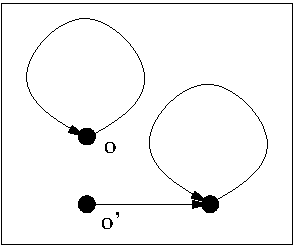
\includegraphics[scale=.8]{pic.pdf}
%\end{center}
%\caption{Distinguishable/indistinguishable points.}\label{fig-car1}
%\end{figure}
%
The individuals $i$ and $i'$ can easily be distinguished in first-order logic:
the formula $R(x,x)$ is true of $i$ and false in $i'$. The corresponding
referring expression for $i$ would be ``an individual relating to itself''.
But if we can only use propositional and relational information (equivalently, our grammar does not contain the word ``itself'') then $i$ and $i'$ are indistinguishable. Both
are ``individuals which are related to individuals which are related to individuals\ldots''

We can connect description logics to the problem of generating
referring expressions via the concept of \emph{bisimulation classes}.
A bisimulation class is a maximal subset $C$ of the domain such that
all members of $C$ are pairwise bisimilar.  For the finite models we
deal with in GRE, this amounts to saying that there are certain
concepts that are satisfied by all individuals in $C$ and no
individuals that are not in $C$ (by Theorems~\ref{bisim}).  If we represent referring expressions as description logic formulas,
this means that there exists a unique referring expression for some
individual $i$ iff $i$ is alone in its bisimulation class; and if it
is, we can use one of the formulas that are characteristic for $C$ as
the referring expression.

Representing referring expressions as DL concepts is a very natural
perspective.  The purely conjunctive set of propositional symbols that,
e.g.,~\newcite{Dale1995} compute is clearly a conjunction in
description logic.  Relational expressions as in
\newcite{dale91:_gener_refer_expres_invol_relat} are concepts of \el.
We will discuss this idea further in Section~\ref{xxx}.

Summing up, we can reduce the problem of computing a unique RE
to the problem of computing the bisimulation classes of a model.  We
will now present two algorithms -- one for \alc\ and one for \el\ --
for doing this.  In fact, each of these algorithms computes all
bisimulation classes of a model at once, effectively computing a RE
for every single individual in the domain simultaneously.


\subsection{Bisimulation classes for \alc and \el}


There exists very efficient algorithms
for computing the bisimulation classes of a model~\cite{hopc:algo71,paig:thre87,dovier04:_effic_algor_for_comput_bisim_equiv}.
These algorithms were originally used for automata minimization: given an
automata $A$ they would return a smaller automata $A'$ which recognized the
same language.  We can adapt these algorithm to compute a formula representing each bisimulation class.  Again, let's first
discuss the $\alc$ case.

We assume given a model $\gM=(\Delta^\gM, |\cdot|^\gM)$ containing all the information about the current
situation.  We will compute a set $\RE$ of $\alc$ formulas such that the
set $\{|\varphi|^\gM \mid \varphi \in \RE\}$ is a partition of $\Delta^\gM$
that contains all the bisimulation classes of $\gM$.  The pseudocode is
shown in Algorithm~\ref{algo:bisim-l} and Algorithm~\ref{algo:bisim-add-alc}.


\begin{theorem}\label{theo:bisimulation-classes}
Given a model $\gM$, the set $\mathcal{C}$ of all $\alc$-bisimulation classes
of $\gM$ is computed by Algorithms~\ref{algo:bisim-l} and~\ref{algo:bisim-add-alc} in polynomial time.  Moreover, for each class $C \in \mathcal{C}$ the algorithm returns an $\alc$ formula $\varphi$ such that
$C = |\varphi|^\gM$.
\end{theorem}

\begin{algorithm}[t]
\dontprintsemicolon
\caption{Computes $\mathcal{L}$-bisimulation classes}
\label{algo:bisim-l}
\KwIn{A model $\gM = (\Delta^\gM, |\cdot|^\gM)$}
\KwOut{A set \RE of formulas  such that
$\{|\varphi|^\gM \in \RE\}$ is the set of $\mathcal{L}$-bisimulation
classes of $\gM$.}

$\RE \leftarrow \{\top\}$

\For{$p \in \prop$}{
      add$_\mathcal{L}(p,\RE)$
   }

\While{for some $\varphi \in \RE, |\varphi|^\gM>1$}{
   \For{$\varphi \in \RE, R \in \rel$}{
         add$_\mathcal{L}(\exists R.\varphi,\RE)$
   }
   \If{made no changes to \RE}{
      exit
      }
}
\end{algorithm}

Algorithms~\ref{algo:bisim-l} and \ref{algo:bisim-add-alc} compute
the \alc-bi\-sim\-u\-la\-tion classes for a given model.
Algorithm~\ref{algo:bisim-l} iterates over all propositional and
relational symbols of the signature to construct new formulas until
either all formulas in $\RE$ denote singletons (i.e., there is only one
individual that satisfies them), or no progress has been made in the
previous iteration.  In each iteration, it calls the procedure
add$_\alc$($\varphi$, $\RE$), which intersects $\varphi$ with any formula $\psi
\in \RE$ which does not denote a singleton and which is
not equivalent to $\varphi$ and to $\neg \varphi$. In this case it
replace $\psi$ in $\RE$ by $\psi \sqcap \varphi$ and $\psi \sqcap \neg \varphi$ to
$\RE$.

The $\alc$ algorithm is driven by case distinctions between
concepts $\varphi$ and $\neg \varphi$, and thus freely adds 
negations to the characteristic formulas in $\RE$.  This can be inconvenient
in natural language generation, because such concepts may be expressible only by rather clumsy natural-language expressions. We will see examples in Section~\ref{xxx}.

An algorithm which is limited to computing
(negation-free) formulas in \el can be obtained by combining
Algorithms~\ref{algo:bisim-l} and~\ref{algo:bisim-add-el}.

As before, the algorithm maintains a set $\RE = \{\varphi_1,\ldots,\varphi_n\}$ of
formulas (this time of \el) such that $\interp{\varphi_1}^\gM \cup \ldots \cup
\interp{\varphi_n}^\gM = \Delta^\gM$, and which it refines iteratively.  However,
where the \alc\ algorithm maintains the invariant that
$\interp{\varphi_1},\ldots,\interp{\varphi_n}$ is a partition of $\Delta$, we
weaken this invariant to the requirement that there are no $m \geq 2$
pairwise different indices $1 \leq i_1,\ldots,i_m \leq n$ such that
$\interp{\varphi_{i_1}} = \interp{\varphi_{i_2}} \cup \ldots \cup
\interp{\varphi_{i_m}}$.  We call the formula $\varphi_{i_1}$ \emph{subsumed} if
such a decomposition exists.

\begin{algorithm}[t]
\caption{add$_\alc(\varphi,\RE)$}
\label{algo:bisim-add-alc}
\For{$\psi \in \RE$ with $|\psi|^\gM > 1$}{
   \If{$|\psi \sqcap \varphi|^\gM \not = \emptyset$ and
       $|\psi \sqcap \neg \varphi|^\gM \not = \emptyset$}{
         add $\psi \sqcap \varphi$ and
               $\psi \sqcap \neg \varphi$ to \RE \;
         remove $\psi$ from \RE \;
      }
   }
\end{algorithm}
%
\begin{algorithm}[t]
\dontprintsemicolon
\caption{add$_\el$($\varphi$, $\RE$)}
\label{algo:bisim-add-el}
\For{$\psi \in \RE$ with $|\psi|^\gM > 1$}{
  \If{$\psi \sqcap \varphi$ is not subsumed in $\RE$ {\bf and}
    $|\psi \sqcap \varphi|^\gM \neq \emptyset$ {\bf and}
    $|\psi \sqcap \varphi|^\gM \neq |\psi|^\gM$}{
    add $\psi \sqcap \varphi$ to $\RE$ \;
    remove subsumed concepts from $\RE$\;
  }
}
\end{algorithm}

The procedure add$_\el$($\varphi$, $\RE$) shown in Algorithms~\ref{algo:bisim-add-el} intersects $\varphi$ with all current formulas in $\RE$
that do not denote a singleton, adds the result to $\RE$ and then
removes all formulas in $\RE$ that have become subsumed.  Removal of
subsumed formulas from $\RE$ can be implemented efficiently by arranging
them by inclusion in terms of their denotation.

\begin{figure*}
  \centering
  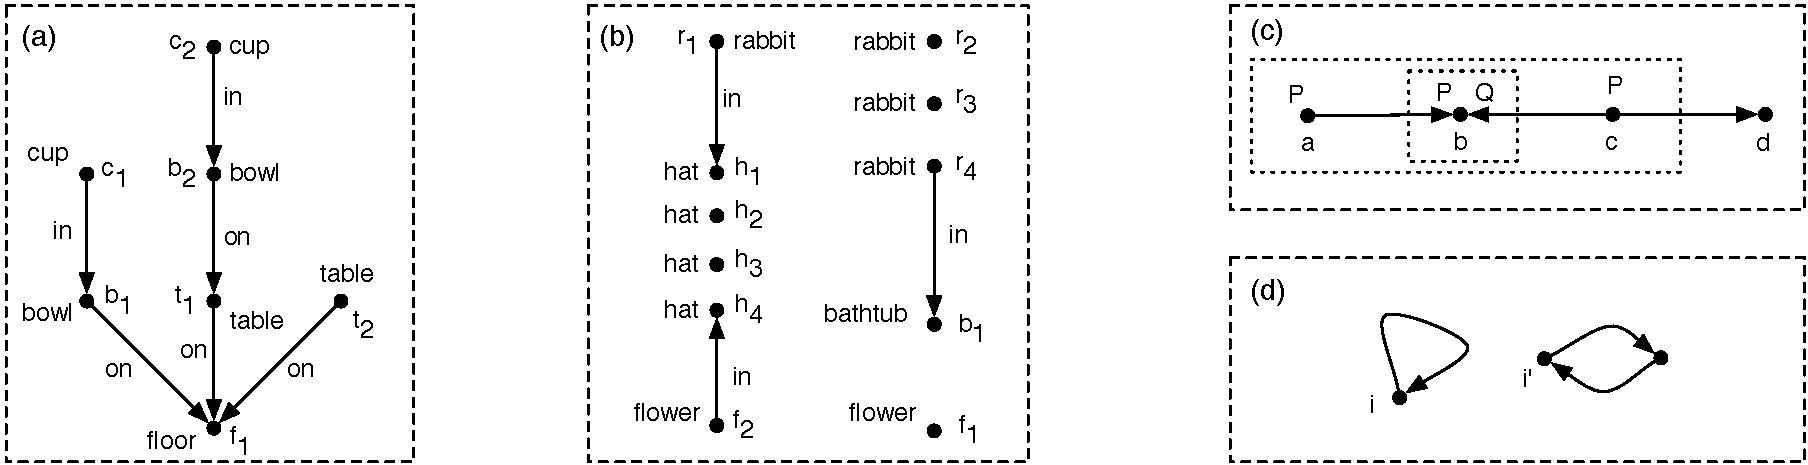
\includegraphics[width=\textwidth]{pic-dale-haddock}
  \caption{(a) The \newcite{dale91:_gener_refer_expres_invol_relat}
    scenario; (b) the \newcite{Stone1998a} scenario; (c) illustrating
    the difference between \el\ and \alc; (d)
    distinguishable/indistinguishable points.}
  \label{fig:dale-haddock}
\end{figure*}

% \begin{figure}
%   \centering
%   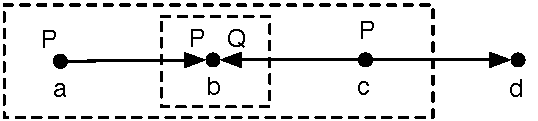
\includegraphics[width=\columnwidth]{pic-el-vs-alc}
%   \caption{Illustrating the difference between \el\ and \alc.}
%   \label{fig:el-vs-alc}
% \end{figure}

\subsection{Some Examples}

Let's see what this algorithm does on the example shown in
Fig.~\ref{fig:dale-haddock}, which is taken from
\newcite{dale91:_gener_refer_expres_invol_relat}.  In the first loop,
the algorithm will add new concepts $\mathsf{floor}$, $\mathsf{bowl}$,
$\mathsf{cup}$, and $\mathsf{table}$; because adding these concepts
makes $\top$ subsumed, $\C$ will consist of these four concepts after
the loop.  Not all of these concepts are singleton; for instance,
$\interp{\mathsf{cup}}$ contains two individuals.  So we iterate over
the relations to make the concepts more precise.  After the first
iteration over the relations, we have $\C = \{ \mathsf{floor},
\mathsf{bowl} \sqcap \exists \mathsf{on}.\mathsf{floor}, \mathsf{bowl}
\sqcap \exists \mathsf{on}.\mathsf{table}, \mathsf{cup},
\mathsf{table} \}$. Notice that $\mathsf{bowl}$ has become subsumed,
but we haven't distinguished the cups and tables further, but we can
use the distinction between the bowls to distinguish the cups in the
second iteration.  The result of this is $\C = \{ \mathsf{floor},
\mathsf{bowl} \sqcap \exists \mathsf{on}.\mathsf{floor}, \mathsf{bowl}
\sqcap \exists \mathsf{on}.\mathsf{table}, \mathsf{cup} \sqcap \exists
\mathsf{in}. (\mathsf{bowl} \sqcap \exists
\mathsf{on}.\mathsf{floor}), \mathsf{cup} \sqcap \exists
\mathsf{in}. (\mathsf{bowl} \sqcap \exists
\mathsf{on}.\mathsf{table}), \mathsf{table} \}$.  At this point, all
concepts except for $\mathsf{table}$ are singleton, and further
iterations don't allow us to refine $\mathsf{table}$; so the algorithm
terminates.  Each of the singleton bisimulation classes is represented
by a characteristic concept; for instance, $\C$ tells us that
$\mathsf{cup} \sqcap \exists \mathsf{in}. (\mathsf{bowl} \sqcap
\exists \mathsf{on}.\mathsf{table})$ is only satisfied by $c_2$, so we
may refer to $c_2$ as ``the cup in the bowl on the table''.

Compared to the \alc\ algorithm, the \el\ algorithm will generally
compute larger bisimulation classes, and compute singleton
bisimulation classes less frequently, because the concepts it can
build can ``see'' fewer differences between individuals.  For example,
in the model shown in Fig.~\ref{fig:el-vs-alc}, the \alc\ algorithm
will compute the concepts $\{\neg \exists R. (\neg P \sqcap \neg Q),
Q, \exists R. (\neg P \sqcap \neg Q), \neg P \sqcap \neg Q\}$ (each of
which is singleton), but $a$ and $c$ are \el-bisimilar in this model,
and the only \el-concept that is true in $d$ is $\top$, so the \el\
algorithm can only compute the concepts $\{\top, P, P \sqcap Q\}$.
Furthermore, because the \el\ algorithm maintains a weaker invariant
for the classes, it may consider more of these classes simultaneously.
Prima facie, this means that it has worst-case exponential runtime,
given that the whole domain has an exponential number of subsets.
However, it is possible that a more careful analysis of the
combinatorics of the considered subsets reveal that the algorithm is
actually polynomial; it certainly behaves polynomially in our
evaluations (see below).


%%% Local Variables: 
%%% mode: latex
%%% TeX-master: "dl-gre-08"
%%% End: 

% \begin{algorithm}[t]
% \dontprintsemicolon
% \caption{\el\ bisimulation classes}
% \label{algo:bisim-el}
% \KwIn{A model $\gM = (\Delta^\gM, |\cdot|^\gM)$}
% \KwOut{A set \RE of pairs $(\varphi,|\varphi|^\gM)$ such that
% $\{S \mid (\varphi,S) \in \RE\}$ is the set of $\el$-bisimulation
% classes of $\gM$.}
% \RE $\leftarrow \{(\top,\Delta^\gM)\}$ \;
% \For{$p \in \prop$}{
%   add$_\el$(p, \RE) \;
% }
% \While{for some $(\varphi,S) \in \RE$, $|S| > 1$}{
%   \For{$(\varphi,S) \in$ \RE, $R \in \rel$}{
%     add$_\el$($\exists R.\varphi$, \RE) \;
%   }
%   \If{made no changes to $\RE$}{
%     exit\;
%   }
% }
% \end{algorithm}